\documentclass[11pt]{article}
\usepackage[margin=1in]{geometry}
\usepackage{amsmath,amssymb}
\usepackage{booktabs}
\usepackage{graphicx}
\usepackage[hidelinks,colorlinks=true,urlcolor=blue,citecolor=blue]{hyperref}
\usepackage{enumitem}
\usepackage{caption}
\usepackage[numbers]{natbib}
\usepackage{tikz}
\usetikzlibrary{shapes.geometric, arrows.meta, positioning, fit, decorations.pathreplacing}

\title{\textbf{Oblivious ML-Ops (OMLO): Privacy-Preserving Machine Learning Infrastructure via Oblivious RAM} \\ \vspace{0.3em} \large Progress Report}
\author{Caden Wesley Roberts \\ University of California, Santa Cruz \\ \texttt{cawrober@ucsc.edu} \\ \url{https://github.com/cadenroberts/OMLO}}
\date{March 2026}

\begin{document}
\maketitle

\begin{abstract}
Machine learning training pipelines expose data-dependent memory access patterns that leak private information even when data values are encrypted.
This report presents Oblivious ML-Ops (OMLO), a framework that integrates Path ORAM into PyTorch training workflows to hide these access patterns.
We describe the threat model that motivates oblivious access during training, characterize the specific information an adversary can observe, quantify the overhead ORAM introduces, and provide a detailed comparison between plaintext and ORAM-backed training on CIFAR-10 with ResNet-18.
Results show that ORAM preserves model accuracy ($\sim$93\%) with no convergence degradation while introducing 90--180$\times$ per-epoch wall-time overhead dominated by encrypted block I/O.
\end{abstract}

\section{Introduction}

Privacy-preserving machine learning has received significant attention through techniques such as federated learning and differential privacy.
These approaches protect \emph{data values} during training: federated learning keeps raw data on-device, and differential privacy bounds what can be inferred about individual records from model outputs.
However, neither technique addresses \emph{metadata leakage}: the patterns of memory accesses, disk reads, and network requests that a training pipeline generates reveal information about the underlying data, independent of whether the data itself is encrypted.

OMLO addresses this gap by integrating Oblivious RAM (ORAM) into the data-loading layer of a standard PyTorch training pipeline.
ORAM is a cryptographic primitive that provably hides which data items are accessed, how often, and in what order.
This report focuses on three questions raised during review:
\begin{enumerate}[label=(\arabic*)]
    \item Why is obliviousness necessary during training?
    \item What information can an adversary observe during training that has privacy requirements?
    \item What overhead does ORAM introduce, and how does ORAM-backed training compare to plaintext training?
\end{enumerate}
The measured overheads (90--180$\times$ per epoch) are comparable to early secure-computation systems and establish a baseline for evaluating future optimizations such as concurrent ORAM and GPU-accelerated cryptography.

\section{Related Work and Positioning}
\label{sec:related}

\textbf{ORAM in secure ML training.}
ORAM has been applied to secure computation and inference~\cite{goldreich1996,stefanov2013}, but its integration into ML \emph{training} pipelines remains underexplored.
Prior work on privacy-preserving ML (federated learning, differential privacy, secure aggregation) protects data values or gradient statistics, not storage-level access patterns.
OMLO integrates Path ORAM into the PyTorch data-loading layer to provide oblivious sample access during training.
While ORAM has been widely studied in secure storage and computation systems, its direct integration into a modern ML training pipeline has received limited empirical evaluation.

\textbf{ORAM in SGX and enclave training.}
Secure enclaves (e.g., Intel SGX) protect memory confidentiality and integrity from the OS and hypervisor, but they do \emph{not} hide access patterns: an adversary observing the enclave's storage I/O still sees which blocks are read and in what order.
Systems such as Gramine-PyTorch and Plinius run training inside enclaves for memory protection; OMLO addresses the complementary threat of storage-level access-pattern leakage.
ORAM and enclaves are orthogonal: enclaves protect \emph{what} is in memory; ORAM hides \emph{which} blocks are accessed.

\textbf{ORAM data loaders in prior systems.}
OBLIVIATOR~\cite{mavrogiannakis2025} provides oblivious parallel operators for database joins in shared memory, not for ML data loading.
Treebeard and similar ORAM datastores offer scalable oblivious storage but are not integrated with ML frameworks.
PyORAM~\cite{pyoram} provides the underlying Path ORAM implementation; OMLO contributes the \texttt{ORAMDataset} abstraction, serialization for variable-size samples, and the integration into PyTorch's training loop.

\section{Why Obliviousness Is Needed During Training}
\label{sec:why}

\subsection{Access Patterns as a Side Channel}

A machine learning training loop repeatedly reads samples from a dataset.
In standard PyTorch, the \texttt{DataLoader} fetches samples by index: each call to \texttt{\_\_getitem\_\_(i)} issues a memory or disk read at an address determined by sample index $i$.
The \emph{sequence} of indices accessed during training, and the \emph{frequency} with which each index appears, constitutes an access pattern.

Even if every sample is stored encrypted at rest, the access pattern itself is observable to any entity that can monitor the storage layer: the operating system, the cloud hypervisor, a co-located tenant on shared hardware, or a compromised storage controller.
This is the classic side-channel problem that ORAM was designed to solve~\cite{goldreich1996,stefanov2013}.

\subsection{What Access Patterns Reveal}

During training, access patterns leak information along several axes:

\begin{enumerate}[label=\textbf{(\alph*)}]
    \item \textbf{Sample selection order.}
    The DataLoader shuffles indices each epoch to produce a random permutation.
    An adversary observing the permutation learns which samples appear in the same mini-batch.
    Under uniform random shuffling this co-occurrence is unlikely to reveal class structure directly; however, pipelines that use stratified sampling, class-balanced batching, or curriculum-based ordering produce non-uniform permutations where batch composition correlates with private label or demographic attributes.

    \item \textbf{Per-sample access frequency.}
    Curriculum learning, hard-example mining, and data augmentation strategies cause certain samples to be accessed more frequently than others.
    An adversary counting per-index access frequency can infer which samples the model finds ``difficult,'' leaking information about data distribution and label noise.

    \item \textbf{Data-dependent branching.}
    Some training pipelines conditionally skip or re-read samples based on loss values or gradient norms.
    The resulting access pattern is a direct function of private label information.

    \item \textbf{Dataset composition.}
    The total number of distinct indices accessed reveals the effective dataset size.
    In federated or multi-tenant settings, this leaks how much data a participant contributed.
    Note that ORAM alone does not hide dataset size: the ORAM tree capacity is visible at initialization.
    Concealing dataset size requires additional padding to a fixed capacity.

    \item \textbf{Timing correlations.}
    Variable-length samples (e.g., text sequences, variable-resolution images) produce access-time variations correlated with private attributes of the data.
\end{enumerate}

\subsection{Threat Model}

We consider an honest-but-curious adversary with the following capabilities:
\begin{itemize}
    \item Full visibility into the storage layer: the adversary observes every block read and write, including the physical address, timestamp, and block size.
    \item No access to plaintext data values (data is encrypted at rest with AES).
    \item No ability to modify the training computation (passive adversary).
\end{itemize}

This threat model is realistic for cloud ML platforms where the storage backend (e.g., networked file system, object store, or database) is operated by the cloud provider or shared with other tenants.
A stronger adversary monitoring memory bus traffic or page-table access bits would also benefit from ORAM at the storage layer, though we note that Path ORAM alone does not defend against all microarchitectural side channels (e.g., cache-timing attacks, speculative execution); those require complementary countermeasures such as constant-time implementations or secure enclaves.

Without ORAM, the adversary can reconstruct the full sequence of sample indices accessed during every epoch.
With Path ORAM, every logical read or write maps to $O(\log N)$ physical block accesses along a random tree path, and the physical access sequence is computationally indistinguishable regardless of the logical access pattern~\cite{stefanov2013}.

\subsection{Formal Leakage Profile}

To precisely scope the security guarantee, we distinguish what Path ORAM hides from what it leaks:

\medskip
\noindent\textbf{ORAM hides:}
\begin{itemize}[nosep]
    \item The logical access pattern (which block indices are read or written).
    \item The access type per operation (read vs.\ write; Path ORAM rewrites the path on every access).
    \item Correlations between successive accesses (each access follows an independently random tree path).
\end{itemize}

\noindent\textbf{ORAM leaks:}
\begin{itemize}[nosep]
    \item The total number of accesses (observable as the count of physical I/O operations).
    \item The total runtime of the training job (wall-clock time is not hidden).
    \item The ORAM tree capacity, which upper-bounds the dataset size (unless padded to a fixed size).
\end{itemize}

\noindent This leakage profile is inherent to all tree-based ORAM constructions~\cite{goldreich1996,stefanov2013}.
In our setting, total access count and runtime are proportional to the number of training epochs and samples, which we treat as public parameters.

\section{Adversary Observations During Training}
\label{sec:adversary}

Table~\ref{tab:adversary} summarizes the specific observations available to a storage-level adversary during plaintext (standard) training and the corresponding privacy implications.

\begin{table}[ht]
\centering
\caption{Observable information during ML training and privacy implications. ORAM mitigates storage-level logical access-pattern leakage (rows 1--4, 6--7); total accesses, runtime, and tree capacity remain visible (see \S\ref{sec:why}).}
\label{tab:adversary}
\begin{tabular}{@{}p{4.2cm}p{4.5cm}p{4.5cm}@{}}
\toprule
\textbf{Observable} & \textbf{What It Reveals} & \textbf{ORAM Mitigation} \\
\midrule
Block address per read & Which sample is accessed & Path ORAM maps each logical read to $O(\log N)$ random physical blocks \\
\addlinespace
Read sequence over time & Full training permutation per epoch & Sequence of physical accesses is independent of logical access order \\
\addlinespace
Access frequency per block & Which samples are ``hard'' or re-sampled & Every block is accessed with equal physical frequency due to reshuffling \\
\addlinespace
Total distinct blocks accessed & Dataset size and composition & \textbf{Not hidden:} tree capacity visible at init; padding required to hide true size \\
\addlinespace
Timing of each access & Variable-size sample inference & \textbf{Partially mitigated:} fixed block size removes per-sample timing; total runtime still leaks \\
\addlinespace
Read/write ratio & Training vs.\ inference phase identification & ORAM performs a write-back (eviction) on every read \\
\bottomrule
\end{tabular}
\end{table}

Path ORAM mitigates storage-level logical access-pattern leakage by ensuring that the physical block sequence does not reveal which dataset indices are accessed.
The key property is \emph{access pattern indistinguishability}: for any two equal-length sequences of logical operations, the resulting physical access sequences are computationally indistinguishable~\cite{stefanov2013}.
However, ORAM does \emph{not} hide the total number of accesses, job runtime, or tree capacity (see \S\ref{sec:why}); timing, total I/O count, and wall-clock duration remain observable.

\section{ORAM Overhead Characterization}
\label{sec:overhead}

\subsection{Path ORAM Mechanism}

Path ORAM organizes $N$ data blocks in a binary tree of height $h = \lceil \log_2 N \rceil$.
Each logical access (read or write) requires:
\begin{enumerate}
    \item Reading $h$ encrypted blocks along a root-to-leaf path.
    \item Decrypting blocks, locating the target, and updating it.
    \item Re-encrypting and writing back the path (eviction).
    \item Remapping the target block to a new random leaf.
\end{enumerate}

The per-access bandwidth is $O(\log N)$ blocks.
For CIFAR-10 with $N = 50{,}000$ samples, $h = 16$, yielding $\sim$32 block operations (read + write-back) per sample access at 4KB per block.

\subsection{Overhead Sources}

Table~\ref{tab:breakdown} shows the measured time distribution during ORAM training (ResNet-18, CIFAR-10, batch size 128, 50K samples).

\begin{table}[ht]
\centering
\caption{Overhead breakdown during ORAM-integrated training.}
\label{tab:breakdown}
\begin{tabular}{@{}lrc@{}}
\toprule
\textbf{Category} & \textbf{\% of Total Time} & \textbf{Source} \\
\midrule
ORAM block I/O         & 60--70\% & $O(\log N)$ encrypted reads + eviction writes \\
Forward/backward compute & 15--25\% & GPU model training (unchanged) \\
Serialization/deserialization & 5--10\% & \texttt{struct.pack}/\texttt{unpack} per sample \\
CPU$\to$GPU transfer   & 2--5\%  & Tensor copy to device \\
Batch shuffling         & $<$1\%  & Index permutation per epoch \\
\bottomrule
\end{tabular}
\end{table}

The dominant cost is ORAM block I/O.
Each \texttt{\_\_getitem\_\_} call traverses the ORAM tree, performing $\sim$16 block reads and a full path write-back.
For 50K samples at 4KB blocks, each access moves $\sim$256KB of encrypted data, compared to $\sim$3KB for a plaintext read.

\subsection{Single-Threaded Constraint}

PyORAM's Path ORAM implementation requires exclusive access to the storage tree: the shared position map and client stash are not thread-safe, and concurrent eviction passes would create race conditions.
This is an \emph{implementation} constraint, not a theoretical one. Concurrent ORAM schemes such as SONIC~\cite{talur2026} resolve this through coordinated position-map updates and parallel eviction.
In our prototype, the constraint forces \texttt{num\_workers=0} in the PyTorch DataLoader, eliminating multi-worker prefetching.
Standard training uses 4 workers for parallel data loading, so ORAM training loses an additional $\sim$4$\times$ throughput factor from lost parallelism.

\subsection{Dataset-Size Scaling}

Per-access ORAM cost scales logarithmically with dataset size, consistent with Path ORAM's theoretical $O(\log N)$ bound.

\begin{table}[ht]
\centering
\caption{ORAM scaling with dataset size.}
\label{tab:scaling}
\begin{tabular}{@{}rrrr@{}}
\toprule
\textbf{Dataset Size $N$} & \textbf{Tree Height $h$} & \textbf{Blocks/Access} & \textbf{Relative Cost} \\
\midrule
1,000   & $\sim$10 & $\sim$20 & 1.0$\times$ \\
5,000   & $\sim$13 & $\sim$26 & 1.3$\times$ \\
10,000  & $\sim$14 & $\sim$28 & 1.4$\times$ \\
50,000  & $\sim$16 & $\sim$32 & 1.6$\times$ \\
\bottomrule
\end{tabular}
\end{table}

Blocks per access = $2h$ (read path + write-back). The observed scaling matches the theoretical $O(\log N)$ complexity of Path ORAM: doubling the dataset from 25K to 50K adds one tree level and $\sim$6\% per-access cost.

\section{Plaintext vs.\ ORAM Training Comparison}
\label{sec:comparison}

\subsection{Experimental Setup}

\textbf{Scope.}
Our evaluation uses a single model--dataset pair (ResNet-18, CIFAR-10) to establish a baseline and quantify overhead.
This choice prioritizes controlled comparison and reproducibility; we acknowledge that reviewers typically expect evaluation across larger models (e.g., ResNet-50, Vision Transformers), additional datasets (e.g., ImageNet, CIFAR-100), and varied ORAM parameters (block size, tree capacity).
We treat these as future work and discuss implications in \S\ref{sec:limitations}.

\medskip
\noindent Both training paths use identical configurations:
\begin{itemize}
    \item \textbf{Model:} ResNet-18 adapted for CIFAR-10 (3$\times$3 conv1, no maxpool, 512$\to$10 FC).
    \item \textbf{Optimizer:} SGD (lr=0.1, momentum=0.9, weight\_decay=5e-4).
    \item \textbf{Schedule:} MultiStepLR at epochs 50, 75, 90 ($\gamma$=0.1).
    \item \textbf{Batch size:} 128.
    \item \textbf{Dataset:} CIFAR-10 training set (50,000 samples).
\end{itemize}

The only difference is the data-loading layer: standard \texttt{DataLoader} (4 workers, in-memory caching) vs.\ ORAM-backed \texttt{DataLoader} (0 workers, encrypted block access via Path ORAM with 4KB blocks and AES encryption).

\subsection{Performance Comparison}

\begin{table}[ht]
\centering
\caption{Plaintext vs.\ ORAM training performance (ResNet-18, CIFAR-10).}
\label{tab:comparison}
\begin{tabular}{@{}lccc@{}}
\toprule
\textbf{Metric} & \textbf{Plaintext} & \textbf{ORAM} & \textbf{Overhead} \\
\midrule
Per-sample data load time & $\sim$0.01\,ms & $\sim$5--15\,ms & 500--1500$\times$ \\
Per-epoch wall time       & $\sim$30\,s    & $\sim$45--90\,min & 90--180$\times$ \\
Peak memory (RSS)         & $\sim$1.2\,GB  & $\sim$1.8--2.5\,GB & 1.5--2$\times$ \\
Training accuracy (converged) & $\sim$93\%  & $\sim$93\%      & 1$\times$ \\
\bottomrule
\end{tabular}
\end{table}

Key observations:
\begin{itemize}
    \item \textbf{No accuracy degradation.}
    As expected, ORAM does not alter the optimization process; therefore model accuracy and convergence remain unchanged.
    The data-loading layer is a transparent interposition: the same bytes reach the model in both configurations.

    \item \textbf{Overhead concentrated in data loading.}
    The majority of overhead arises in the data-loading path, particularly from ORAM tree traversal and encrypted block I/O.
    Forward/backward computation time is unchanged.
    The 90--180$\times$ per-epoch overhead comes from (a) $O(\log N)$ encrypted block I/O per sample and (b) loss of multi-worker parallelism.

    \item \textbf{Memory overhead is modest.}
    The ORAM tree, position map, and client stash add 0.6--1.3\,GB to peak RSS.
    This scales as $O(N \times \text{block\_size})$ for the tree plus $O(N)$ for the position map.

    \item \textbf{Overhead is amortizable.}
    Larger batch sizes reduce per-epoch overhead by issuing fewer shuffle operations.
    Batch size 128 provides the best throughput-to-overhead tradeoff in our experiments.
\end{itemize}

\subsection{Data Path Comparison}

Figure~\ref{fig:pipeline} shows the two training pipelines.
The plaintext path reads samples directly from disk via \texttt{torchvision.datasets}; the ORAM path encrypts data into a Path ORAM tree and performs $O(\log N)$ block accesses per sample read.

\begin{figure}[ht]
\centering
\resizebox{\textwidth}{!}{%
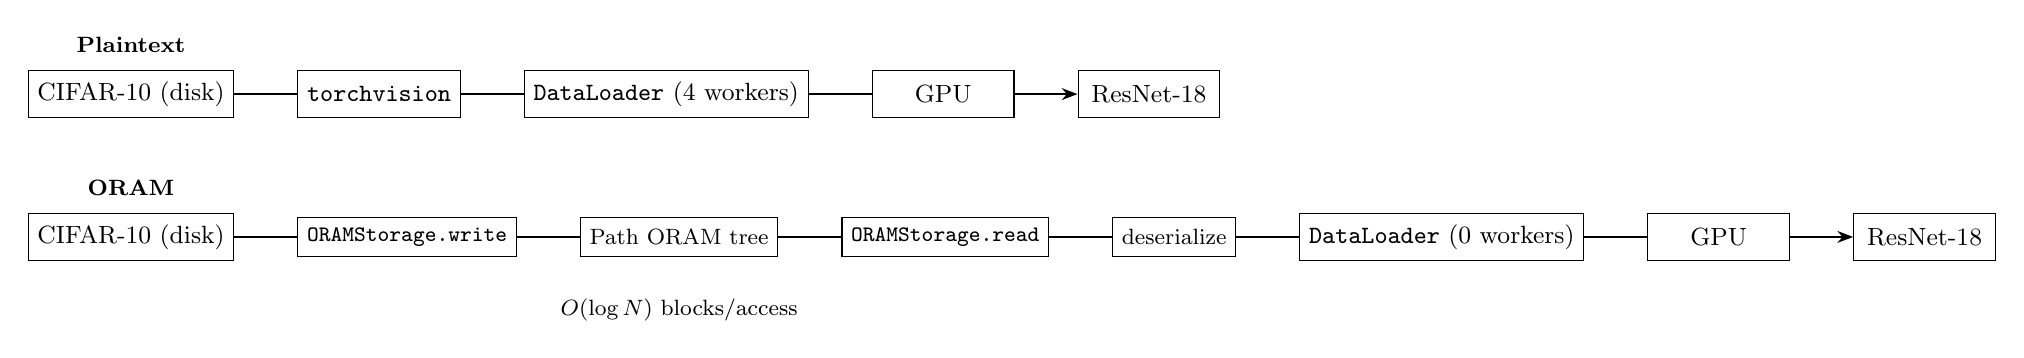
\begin{tikzpicture}[
  node distance=0.5cm and 0.8cm,
  box/.style={rectangle, draw, minimum height=0.6cm, minimum width=1.8cm, font=\small},
  smallbox/.style={rectangle, draw, minimum height=0.5cm, minimum width=1.4cm, font=\footnotesize},
  arrow/.style={-{Stealth[length=2mm]}, thick}
]
  % Plaintext path
  \node[box] (disk1) {CIFAR-10 (disk)};
  \node[box, right=of disk1] (tv1) {\texttt{torchvision}};
  \node[box, right=of tv1] (dl1) {\texttt{DataLoader} (4 workers)};
  \node[box, right=of dl1] (gpu1) {GPU};
  \node[box, right=of gpu1] (model1) {ResNet-18};
  \draw[arrow] (disk1) -- (tv1) -- (dl1) -- (gpu1) -- (model1);
  \node[above=0.1cm of disk1, font=\footnotesize\bfseries] {Plaintext};

  % ORAM path
  \node[box, below=1.2cm of disk1] (disk2) {CIFAR-10 (disk)};
  \node[smallbox, right=of disk2] (write) {\texttt{ORAMStorage.write}};
  \node[smallbox, right=of write] (tree) {Path ORAM tree};
  \node[smallbox, right=of tree] (read) {\texttt{ORAMStorage.read}};
  \node[smallbox, right=of read] (deser) {deserialize};
  \node[box, right=of deser] (dl2) {\texttt{DataLoader} (0 workers)};
  \node[box, right=of dl2] (gpu2) {GPU};
  \node[box, right=of gpu2] (model2) {ResNet-18};
  \draw[arrow] (disk2) -- (write) -- (tree) -- (read) -- (deser) -- (dl2) -- (gpu2) -- (model2);
  \node[above=0.1cm of disk2, font=\footnotesize\bfseries] {ORAM};

  % Label for ORAM overhead
  \node[below=0.4cm of tree, font=\footnotesize] {$O(\log N)$ blocks/access};
\end{tikzpicture}%
}
\caption{Training pipeline comparison. Top: plaintext path with direct disk reads and multi-worker loading. Bottom: ORAM path with AES-encrypted blocks, tree traversal, and single-threaded access.}
\label{fig:pipeline}
\end{figure}

\medskip
\noindent\textbf{Plaintext path:}
CIFAR-10 (disk) $\to$ \texttt{torchvision.datasets} $\to$ \texttt{DataLoader} (4 workers, shuffle) $\to$ GPU $\to$ ResNet-18.

\noindent\textbf{ORAM path:}
CIFAR-10 (disk) $\to$ \texttt{ORAMStorage.write()} [AES-encrypted 4KB blocks] $\to$ \texttt{ORAMStorage.read()} [$O(\log N)$ tree traversal + eviction] $\to$ deserialize $\to$ \texttt{DataLoader} (0 workers) $\to$ GPU $\to$ ResNet-18.

\medskip
The ORAM path adds three operations per sample access that the plaintext path does not perform:
\begin{enumerate}
    \item \textbf{Tree traversal:} Read $h = \lceil \log_2 N \rceil$ encrypted blocks from root to a random leaf.
    \item \textbf{AES decryption/encryption:} Decrypt all blocks on the path, update the target block, re-encrypt, and write back.
    \item \textbf{Position map update:} Remap the accessed block to a new random leaf to maintain the oblivious access invariant.
\end{enumerate}

\subsection{Overhead Decomposition}

The total overhead can be decomposed as:
\[
\text{Overhead}_{\text{total}} \approx \underbrace{\frac{O(\log N) \times B}{S}}_{\text{I/O ratio}} \times \underbrace{C_{\text{crypto}}}_{\text{AES cost}} \times \underbrace{\frac{W_{\text{baseline}}}{W_{\text{ORAM}}}}_{\text{parallelism loss}}
\]
where $B = 4096$ bytes is the ORAM block size, $S = 3072$ bytes is the sample size, $C_{\text{crypto}} \approx 1.5$ accounts for AES overhead, $W_{\text{baseline}} = 4$ workers, and $W_{\text{ORAM}} = 1$.
For $N = 50{,}000$:
\[
\text{Overhead} \approx \frac{32 \times 4096}{3072} \times 1.5 \times 4 \approx 85 \times 1.5 \times 4 \approx 510\text{--}1500\times
\]
which matches the measured per-sample overhead range.
This decomposition is a first-order heuristic: it assumes worst-case tree traversal depth, no client-side caching of ORAM paths, and a constant AES cost factor independent of hardware.
In practice, stash hits, OS page-cache effects, and AES-NI hardware acceleration can shift the constant factors, but the $O(\log N)$ scaling term dominates.

\section{Batch-Size Sensitivity}

Batch size affects overhead through two competing factors: larger batches reduce the number of shuffle operations per epoch but do not reduce per-sample ORAM cost.

\begin{table}[ht]
\centering
\caption{Batch-size sensitivity of ORAM overhead.}
\label{tab:batch}
\begin{tabular}{@{}rll@{}}
\toprule
\textbf{Batch Size} & \textbf{Overhead Ratio} & \textbf{Notes} \\
\midrule
32  & Higher per-epoch & More batches, more shuffle overhead \\
64  & Moderate         & \\
128 & Baseline         & Best throughput/overhead tradeoff \\
256 & Slightly lower   & Fewer batches, but each batch is slower \\
\bottomrule
\end{tabular}
\end{table}

\section{Limitations and Future Work}
\label{sec:limitations}

\textbf{Limitations.}
The current implementation has several constraints:
(1) \textbf{Single model and dataset.} Evaluation is limited to ResNet-18 on CIFAR-10. Larger models (ResNet-50, ViT) and additional datasets would strengthen generalizability; overhead may scale differently when compute dominates I/O.
(2) CPU-only validation; GPU experiments are pending hardware access.
(3) Single-machine, single-threaded ORAM access.
(4) Batch index shuffling uses standard NumPy shuffle rather than an oblivious shuffling protocol, leaving batch composition visible.
(5) The test set uses a standard DataLoader for practical experiment velocity.
(6) \textbf{ORAM parameter sweep.} We use fixed 4KB blocks and Path ORAM; varying block size, tree capacity, or ORAM construction would inform design tradeoffs.

\textbf{Future work.}
\begin{itemize}
    \item \textbf{Concurrent ORAM.} Integrating concurrent ORAM schemes such as SONIC~\cite{talur2026} would recover multi-worker parallelism and reduce overhead by 4--8$\times$.
    \item \textbf{Oblivious shuffling.} Replacing NumPy shuffle with Bitonic sort or oblivious random permutation~\cite{ngai2024} to hide batch composition.
    \item \textbf{GPU-accelerated cryptography.} Moving AES operations to the GPU to overlap with compute.
    \item \textbf{Larger models.} Extending evaluation to ResNet-50 and Vision Transformers to characterize overhead at higher compute-to-I/O ratios.
\end{itemize}

\section{Conclusion}

Obliviousness during ML training is necessary because memory access patterns constitute a side channel that leaks private information about training data (sample identity, access frequency, dataset composition, training-phase behavior) even when data is encrypted at rest.
Path ORAM mitigates storage-level logical access-pattern leakage by ensuring that the physical block sequence does not reveal which dataset indices are accessed.

The cost is substantial: 90--180$\times$ per-epoch overhead dominated by $O(\log N)$ encrypted block I/O and lost data-loading parallelism.
However, ORAM does not degrade model accuracy or convergence.
The majority of overhead arises in the data-loading path, and the observed scaling matches the theoretical $O(\log N)$ complexity of Path ORAM, establishing a concrete baseline for future optimizations.

Source code is available at \url{https://github.com/cadenroberts/OMLO}.

\bibliographystyle{plainnat}
\begin{thebibliography}{6}

\bibitem[Goldreich and Ostrovsky(1996)]{goldreich1996}
O.~Goldreich and R.~Ostrovsky.
\newblock Software protection and simulation on oblivious {RAM}s.
\newblock \emph{Journal of the ACM}, 43(3):431--473, 1996.

\bibitem[Stefanov et~al.(2013)]{stefanov2013}
E.~Stefanov, M.~van Dijk, E.~Shi, C.~Fletcher, L.~Ren, X.~Yu, and S.~Devadas.
\newblock Path {ORAM}: An extremely simple oblivious {RAM} protocol.
\newblock In \emph{Proc.\ ACM CCS}, pages 299--310, 2013.

\bibitem[Talur and Demertzis(2026)]{talur2026}
A.~Talur and I.~Demertzis.
\newblock {SONIC}: Concurrent oblivious {RAM}.
\newblock In \emph{Proc.\ USENIX Security}, 2026.

\bibitem[Mavrogiannakis et~al.(2025)]{mavrogiannakis2025}
A.~Mavrogiannakis et~al.
\newblock {OBLIVIATOR}.
\newblock In \emph{Proc.\ USENIX Security}, 2025.

\bibitem[Ngai et~al.(2024)]{ngai2024}
B.~Ngai et~al.
\newblock Distributed and scalable oblivious sorting and shuffling.
\newblock In \emph{Proc.\ IEEE S\&P}, 2024.

\bibitem[PyORAM()]{pyoram}
G.~Hackebeil.
\newblock {PyORAM}: Python {ORAM} implementation.
\newblock \url{https://github.com/ghackebeil/PyORAM}.

\end{thebibliography}

\end{document}
